\documentclass{beamer}
% \usepackage{C:/SystemFiles/tinytex/tex/rfaye3}
\usetheme{Malmoe}
\usepackage{ctex}% 中文环境
\usepackage{cite}
\AtBeginSection[]
{
  \begin{frame}{概述}
    \tableofcontents[currentsection]
  \end{frame}
}

\begin{document}


\author{任永文}%作者
\title{报告题目:毕业设计调研(三)}%演讲题目
\frame{\titlepage}

% \begin{frame}{目录}
%   \setbeamertemplate{section in toc}[sections numbered]
%   \tableofcontents[hideallsubsections]
% \end{frame}

\begin{frame}{Data Preptarion}
  Dataset
  \begin{enumerate}
    \item common\_language\_kpd
    \item musan
    \item rir\_noises
  \end{enumerate}
  Data Augmentation
  \begin{enumerate}
    \item Mixture of non-speech noises(music noise babble), which are from MUSAN
    \item Reverbation injection, using sitmulated impulse responses from RIR\_NOISES
    \item SpecAugmentation
  \end{enumerate}
\end{frame}

\begin{frame}{System Description}
  \begin{enumerate}
    \item features: Fbank
    \item baseline: ecapa-tdnn
    \item classifier: 192 to 45
    \item finetune: adam + ce-loss/aam-softmax
  \end{enumerate}
  \begin{figure}
    \centering
  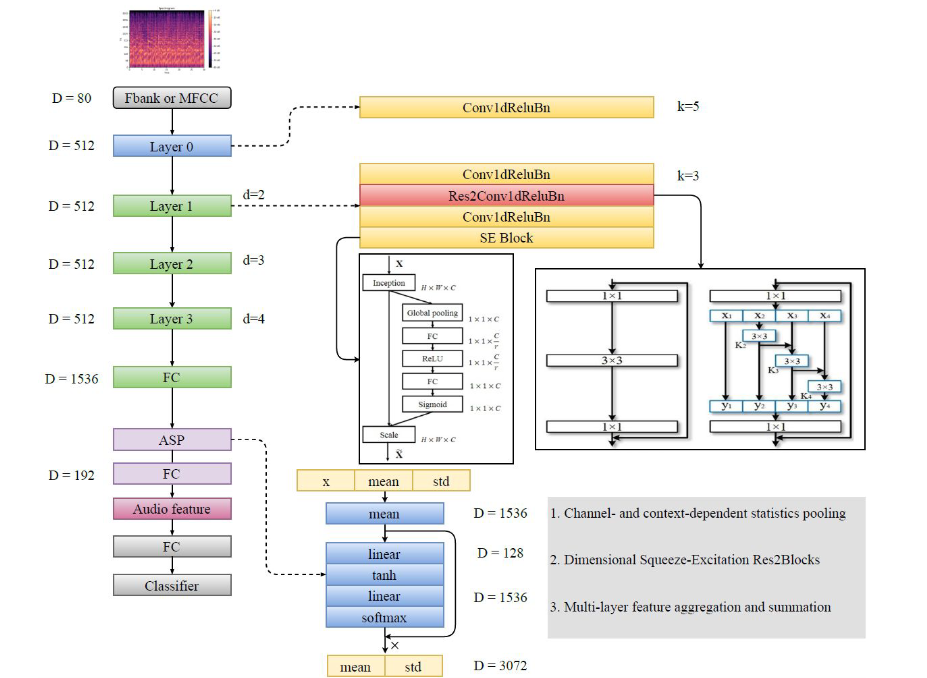
\includegraphics[width=0.8\textwidth]{image/2-0.png}
  \end{figure}
\end{frame}

\begin{frame}{Experiment settings}
  \begin{enumerate}
    \item input features:resample to 16000Hz, 80-dim fbank
    \item model settings:(channels:[1024,1024,1024,1024,3072], attention\_channels:128, output:192)
    \item train strategies: lr:1e-4, lr\_decay:0.97, batch\_size:64
  \end{enumerate}
\end{frame}

\begin{frame}{Experiment results}
  \begin{figure}
    \centering
  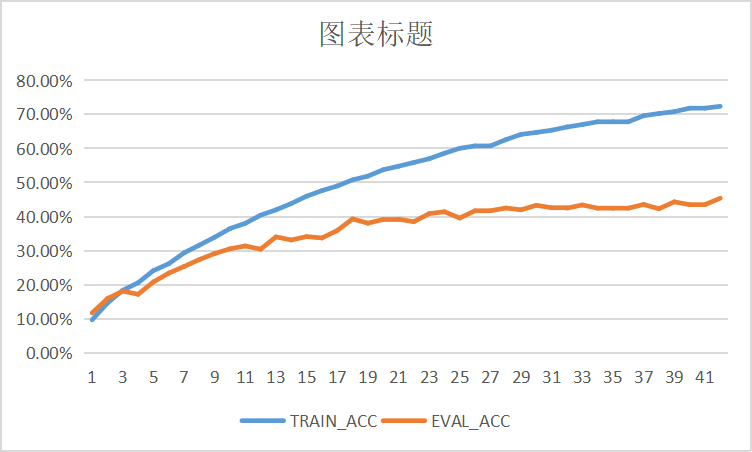
\includegraphics[width=0.45\textwidth]{image/3-1.png}
  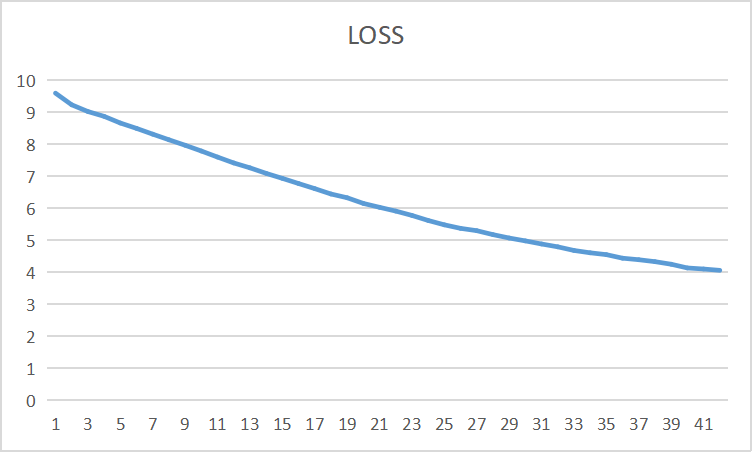
\includegraphics[width=0.45\textwidth]{image/3-2.png}
  \end{figure}
  \begin{table}[]
    \begin{tabular}{|l|l|l|l|l|}
    \hline
    loss\_function                & lr            & batch & loss            & acc                       \\ \hline
    crossentropy                  & 1e-3          & 64          &                 & 65\%                      \\ \hline
    aam+crossentropy       & 1e-3          & 64          &slowly &                           \\ \hline
    aam+kldiv          & *             & 4           &slowly &                           \\ \hline
    aam+kldiv         & 1e-3          & 64          &                 & rise then decline \\ \hline
    \textbf{aam+kldivloss} & \textbf{1e-4} & \textbf{64} & \textbf{}       & \textbf{45\%}             \\ \hline
    aam+kldiv+pretrain & 1e-4          & 64          &well    & 65\%+                     \\ \hline
    \end{tabular}
    \end{table}
\end{frame}

\appendix
\section<presentation>* {\appendixname}
\subsection<presentation>{For Further Reading}
\begin{frame}[allowframebreaks]
  \frametitle<presentation>{For Further Reading}
  \begin{thebibliography}{10}
    \beamertemplatebookbibitems
    \bibitem{Author1990}  TaoRuijie,speechbrain
    \newblock {\em ECAPA-TDNN}.
    \newblock https://github.com/TaoRuijie/ECAPA-TDNN
    \newblock https://github.com/speechbrain/speechbrain
  \end{thebibliography}

\end{frame}
\end{document}

